\documentclass[conference]{IEEEtran}

\usepackage[pdftex]{graphicx}

\hyphenation{op-tical net-works semi-conduc-tor}

\begin{document}

\title{Translating C concurrent programs to UPPAAL timed automatas: An automated approach.}

%\author{\IEEEauthorblockN{Pablo Gonzalez-de-Aledo, Alvaro Diaz, Pablo Sanchez}
%\IEEEauthorblockA{GIM, TEISA \\
%University of Cantabria\\
%39005 Santander, Cantabria, Spain\\
%Email: \{pabloga,adiaz,sanchez\}@teisa.unican.es }
%}
\author{\IEEEauthorblockN{}
\IEEEauthorblockA{\\
\\
\\
}
}

\maketitle

\begin{abstract}
This paper describes a methodology and tool that translates to UPPAAL diagrams concurrent C programs that use the POSIX ``pthread'' library to provide parallelism. This  methodology enables the UPPAAL solver to evaluate real implementations of  the  intended  design  instead  of  an  early  system-level version. It also has the benefit that the same verification engine is used in a top-down and bottom-up approach. UPPAAL is a well-known verification framework that provides a graphical-user interface to represent the timed automatas that are used for the verification. Besides the benefits of formal verification of concurrent C programs, the ability to see these timed automatas that represent C functions can be useful for validation and debugging.
%This paper describes the design and implementation of a tool that translates concurrent programs described in C and using the pthread library to UPPAAL diagrams. This flow enables the UPPAAL engine to reason about a real implementation of the intended design instead of an early simplified version, and has the benefit that the same verification engine is used in a top-down and bottom-up approach. UPPAAL has been selected because of its popularity and the fact that it provides a graphical-user interface to represent the timed automatas that are used for the verification. Besides the benefits of formal verification of concurrent C programs, the ability to see these timed automatas that represent C functions can be useful for teaching purposes and debugging.
\end{abstract}

\IEEEpeerreviewmaketitle

\section{Introduction}

Embedded systems are constantly growing in number and complexity around us. They are responsible of our security, our health, environmental issues... Because of their ubiquity and importance, there is a great interest both in industry and academia in developping efficient techniques to verify them.

Currently, verification is done with manually generated testcases. Such testing accounts for 50-­80\% of the cost of embedded software development. Also, manual testing is error ­prone, time ­consuming, expensive and rarely efficient enough. This causes that, despite all the effort in software quality assurance, serious code defects are routinely discovered, leading to vulnerabilities, increasing cost and loosing of credibility for enterprises.

Most software is nowadays running in parallel with other software components, especially because SoCs natively support concurrency. This leads to new problems that previously did not exists to such an extreme:

\begin{itemize}
    \item Defects on concurrent software are hard to understand and errors commonly comes from the subtle interaction between different portions of code executing in parallel. Therefore, deep knowledge about the program and these parellel interactions is needed to debug concurrent software.
    \item The number of possible interactions between threads increases exponentially with the number of threads and the size of parallel code. However, the vast majority of those interactions are benign, and only an infinitesimal fraction of them cause real errors, so finding those corner cases is like finding a needle in a haystack.
    \item The program output of a concurrent program depends not only on inputs but also on the execution order of different tasks. Since this ordering is different every time the program is executed, errors are very difficult to reproduce, and it is likely that they do not show until very advanced phases of design, or even in production. The non-­determinism makes the system very difficult to be debugged, as the execution that leads to an error can not easily be replicated.
\end{itemize}

Despite all those difficulties, it is likely that all software will be parallel in the near future. Limitations in power dissipation, power consumption and execution time impede further development of programs without parallelization. However, there's not a complete solution today to effectively test concurrent programs.

A frequently used approach to deal with these difficulties is the following one:

\begin{enumerate}
    \item First, a high-level abstracted model for the application is performed. These models are similar to the one presented in Figure \ref{simple_philo} , and are commonly done by hand using the information obtained from a verbal description of the application requirements.
    \item This model is progressively refined to a implementation, generally written in some programming language. A commonly used programming language for embedded systems is C/C++ with the pthreads library as a way of modeling concurrency. This implementation is generally similar to the one presented in Figure \ref{fig:philosophers}. Note that the flow has been heavily altered between the initial description and the final implementation.
\end{enumerate}


\begin{figure}[b!]
\centering
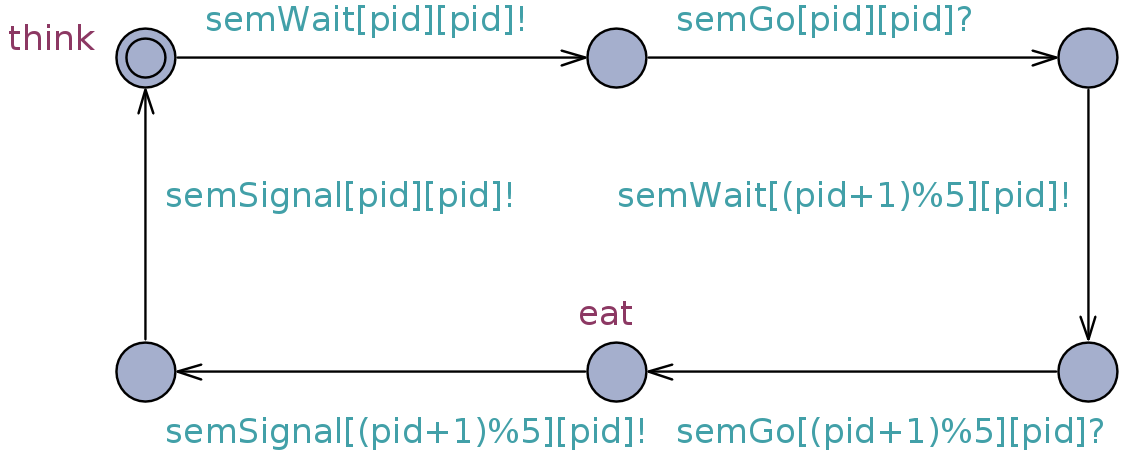
\includegraphics[width=0.75\columnwidth]{media/simple_philo.png}
\caption{Simple UPPAAL model}
\label{simple_philo}
\end{figure}

Some of the problems associated with this flow are:

\begin{itemize}
    \item The refinement process is done manually, and there is no guarantee that the implementation is indeed equivalent to the high-level model.
    \item There exists tools that can reason about high-level models (i.e. UPPAAL \cite{uppaal}), and different tools that can reason about actual implementations (i.e. CBMC \cite{cbmc}, SAGE \cite{sage}), but generally, different tools are not integrated together, so proving that actual implementation also complains with high-level properties is not trivial.
    \item Also caused by the different frameworks used for different levels of abstraction, the queries needed to verify the actual implementation are different to the ones used to verify the implementation.
    
    \item The semantic of synchronization procedures of the initial model (atomic actions, signals...) has to be transformed to the primitives of the target language (mutexes, mutexs, monitors...). These transformations can cause the final implementation to be incorrect despite the fact that the idealized model is correct. To make the semantic gap between the model and the implementation smaller, the former is usually designed with implementation in mind, and the transformation process is driven by the particular implementation.
    
\end{itemize}

This paper presents a tool that automatically translates from C to UPPAAL models. This enables the UPPAAL engine to reason about an actual implementation instead of a high-level view of the system. The tool keeps coherent names for the variables in the C code, so the same queries that are performed to the high-level implementation of the system can be performed to the resulting model that is outputted by the tool.

\section{State of the Art}

As commented in the introduction, it is indubitable that applications need to be concurrent to fully exploit CPU throughput gains. However, improper use of locks may lead to race conditions, deadlocks or starvation. For this reason it is important to verify concurrency in the final implementation. 

Previous research in this area has focused on obtaining correct C implementations `by construction'. Under these approaches, we can find several tool that translate UPPAAL models to source code (specification  down to implementation) \cite{pedersen}\cite{hendriks01}\cite{amnell04}. These tools have the disadvantage that the semantic of the generated code is limited, so the code is difficult to understand and developers are reluctant to accept this flow. On the other hand, some approaches \cite{cicirelli2011} have been proposed to translate source code to UPPAAL (implementation up to specification). To the knowledge of the authors, however, these approaches are always manual and therefore tedious and error prone.

Paper \cite{pajik11} presents a framework  that facilitates automatic conversion of verified models (in UPPAAL) to models that may be simulated and tested (in Simulink/Stateflow). Another work from specification  down to implementation is presented in \cite{pedersen} where authors proposes a translation from a UPPAAL model to an implementation written in C. For this translation, the UPPAAL model need a previous deterministic semantic simplification.
In \cite{hendriks01} authors present a translation from UPPAAL models of real-time controllers to NQC (Not-Quite C) programs.

Relating the other approach (implementation up to specification), \cite{cicirelli2011} proposes an approach for modelling and verifying concurrent programs targeted to be implemented in Java using UPPAAL. Another similar aproach is presented in \cite{cicirelli13} where authors describe a library of UPPAAL timed automata reproducing the semantic of major Java concurrent and synchronization mechanisms, which fosters a smooth transition from specification down to implementation.

The approach described in this paper is fully automatic, in contrast with these last two references where a user must manually connect the synchronization elements to archieve the desired functionality. On the other hand, the flow still preserves the goal of visually help the developper to understand the synchronization of the application under test. This leads to different synchronization primitives as the ones described in \cite{cicirelli2011}\cite{cicirelli13}. While the goal of the two approaches is to mimic the behaviour of C/Java synchronization elements, \cite{cicirelli2011}\cite{cicirelli13} have focused more on efficiency (both in verification time and memory), while this work focuses more on simplicity of the generated graph.

% más referencias

%This paper contribution can be related to the solutions
%proposed e.g. by Hamberg & Vaandrager in [7] and to the
%well-known approach FSP/LTSA [8]. 



%On-going and future work are geared to:
%• Optimizing the library so as to improve the efficiency of
%model checking activities.
%• Extending the library with other concurrency control
%structures, e.g. based on the concept of software trans-
%actional memory [14] which delivers a different and
%attractive style of concurrent programming.
%• Extending the approach based on the U PPAAL model
%checker to M&V of lock-free concurrent objects [14]
%which are often perceived as a grand challenge for an
%exploitation, in parallel and embedded software systems,
%of the computing potential of current and future multi-
%core/many core machines.

\section{Modeling}

\subsection{Modeling of the whole system}

To reason about a concurrent system, the whole program is considered to be a set of timed automata. The methodology and the tool presented in this paper are meant to be used to reason about the concurrent part of the system, and therefore all the functionality that is not executed in parallel to another function is not considered in the analysis. The user must provide indications of which function he wants to analyse (i.e. which functions can be executed in parallel as the effect of calling pthread\_create). This information could also be obtained by symbolically analyse the pointers to functions passed to `pthread\_create' functions, as discussed in section `future work'.

\subsection{Modeling of each timed automata}

Each function involved in the parallel section of the code can be modelled as a timed automaton. This automaton is composed of the following elements:

\begin{description}
    \item [$S$: ] A finite set of states
    \item[$S_0$:] A initial state
    \item[$A$:  ] A finite set of actions
    \item[$\tau$:] $S \times A \rightarrow S$: a partial transition function
    \item[$\Pi$:] A finite set of boolean propositions
    \item[$L$:] $S \rightarrow 2^\Pi$ A labeling function
\end{description}


UPPAAL adds to the previous elements the notion of ``urgent'' states ($U: S \rightarrow \{'normal', 'urgent', `commited'\}$), that enables to consider certain states to be expugned from the scheduling algorithm (i.e. all `urgent' and `commited' states are executed together, without the possibility of being interrupted by another timed automaton), so the solving algorithm for different interleavings can be simplified.

There are several difficulties in the translation of a high-level programming language to this timed automaton:

\begin{itemize}
    \item [a] The notion of 'state' is not clearly defined in the high-level programming language.
    \item [b] Actions has a much richer semantic in the high-level language than in the UPPAAL model (i.e. actions might imply pointers, arrays, function calls, structures, unions, ternary operator ...)
    \item [c] mutexs are commonly used via dynamic dereference of pointers in the code, so $\tau$ is not a statically defined function, but instead it depends on dynamic user data.
    \item [d] Transition functions are required to be side-effect free in the UPPAAL description, while a mutex has inherently the side-effect of locking/unlocking the synchronization element.
\end{itemize}

\subsection{Modeling of the synchronization elements}

This section describes the design of the basic synchronization element generated by the tool. 

A key element of the translation methodology described in this paper is the instantiation of synchronization elements that arbitrate the execution of different timed automata. This synchronization element is based in pthread's `mutex' datatype, which has been chosen because of the following reasons:

\begin{itemize}
    \item It complies with the two requirements of a proper mechanism to arbitrate access to shared data by multiple processes \cite{philo_1}
    \begin{itemize}
        \item It must guarantee that only one process at a time can access shared data
        \item It provides a method that enables an automaton to suspend its execution when the condition needed to complete the operation does not met.
    \end{itemize}
    \item All other synchronization mechanisms (mutexs, critical sections, monitors...) can be implemented by means of mutexes.
\end{itemize}

 

\section{Implementation}

This section describes the solution to the problems mentioned in subsection B of the previous section:

\subsection{Notion of state}

Depending on the target of the UPPAAL diagram, the tool enables two different notions of state:

\begin{itemize}
\item In `synchronization-mode', states are considered to be only the calls to lock/unlock functions.
\item In `full-mode', states are defined as the lock or unlock of a mutex in the C code, or every conditional branch of the code. Locking/unlocking are non-urgent states. Conditionals are urgent if they depend on `global' data (i.e. data that can be modified by another thread).
\end{itemize}

This two different notions of state are targeted to two different purposes of the UPPAAL diagram:

\begin{itemize}
\item `Synchronization-mode' is meant to be used to visually represent the parallel functions of the C code. Only calls to pthread lock/unlock functions are considered states, which leads to very compact graphs that are similar to the high-level representation. These graphs can be used in a first step in verification, as a visual guidance to check that the implementation has the same behaviour than the intended high-level model
\item In `full-mode', conditional branches (i.e. \verb+if+, \verb+switch+, \verb+ternary operator+, \verb+for+, \verb+while+, \verb+do+ ...) are also considered states, which usually leads to much bigger graphs and higher verification times. However, the real synchronization is being modeled, and this mode enables to detect potential bugs caused by race conditions.
\end{itemize}

\subsection{High-level language semantic}

To simplify the semantic of the high-level language, the framework uses symbolic execution to cover all possible paths in the code while the program is symbolically executed. A few stubs have been added to the symbolic execution framework to be able to reduce the input semantic to a smaller set of operations:

\begin{itemize}
    \item Binary instructions
    \item Pointer dereferences
    \item Assignments
    \item Conditionals
\end{itemize}

Some of the complexity of high-language semantic are simplified by LLVM \cite{llvm} transformation passes (e.g. unification of conditional branch statements (\verb+do-while+, \verb+for+, \verb+if+, \verb+switch+,\verb+?:+, \verb+while+, ...)), while others are simplified when the program is executed (i.e. function-calls or concretization of pointer dereferences, as explained in the next section).

\subsection{Dynamic dereference of pointers to mutexs}

The use of symbolic execution enables the framework to reason about all possible values for a pointer in the moment that pointer is dereferenced. When the pointer that is being dereferenced points to a \verb+pthread_mutex_t+ object, the symbolic execution framework generates a case split, producing new transitions ($\tau'$(uppaal partial transition function)$: S \times A' \rightarrow S$) where $A'$ is the proposition $variables\_that\_might\_affect\_the\_pointer == value$. (see Figure \ref{fig:case_split}). To be able to generate this case-split, both the set of affecting variables and the base and extension of each created array are tracked by the symbolic execution framework. The set of assignments for affecting variables is then generated by iteratively solving the SMT equation $base \leq expression\_of\_pointer \leq base + extension$.


\begin{figure}
\centering
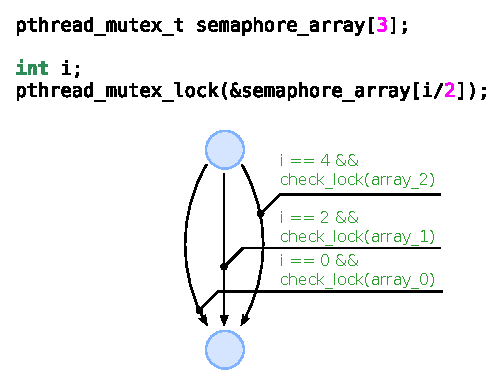
\includegraphics[width=0.75\columnwidth]{media/case_split.pdf}
\caption{Transformation of a pointer to mutex in a case-split}
\label{fig:case_split}
\end{figure}

\subsection{side-effect-free synchronization elements}

To make the transition function side-effect, it is split in two functions: \verb+check_function+ and \verb+update_function+. The \verb+check_function+ forms part of the guard, while the \verb+update_function+ is included among the actions of the transition.

The mutexes are implemented based on functions that operate modifying the fields of a UPPAAL structure `Mutex'. This structure is passed by value to the \verb+check_+ function and by reference to the \verb+update_+ function. The \verb+check_+ function is used in the `guard' of the transition, while the \verb+update_+ function is used in the update field of the transition. The purpose of the check function is to prevent the execution and evaluate in the guard the status of the mutex. This \verb+check_+ function indicates when the mutex is free to lock/unlock and enables the transition between locations. As it is explained previously, the expression guard in UPPAAL must be side-effect free and it cannot modify the value of the mutex. This is the reason why it is needed to use the \verb+update_+ function in the update expression of the same transition. This function has the side-effect of updating the mutex value.


\subsection{Symbolic execution}


To symbolically execute the code, we use the `Forest' framework \cite{forest_tacas}. This framework is divided in several stages that are described below:

\begin{itemize}
	\item Front-End:  As front-end we use the LLVM framework, that transforms the C code to llvm intermediate representation. 
	\item Optimization-passes: Several optimization passes reduces the semantic of llvm intermediate representation to more concrete operations (e.g. ternary operator or switchs are transformed to if statements, structure accesses are transformed to pointer dereferences ...). More flattening is produced when the program is run (step 5). 
	\item Anotation: An optimization pass is applied to the intermediate representation, so every operation is instrumented with calls to back-end functions.
	\item Linking: The intermediate representation is linked with the verification library. This library implements the every operation performed in the intermediate representation and evaluates these operation during symbolic execution as explained in the following step.
	\item Execution: When executed, the program forks on every condition encountered in execution. While the program is run, the inserted stubs compute an SMT formula for each variable, and this formula is passed to a SMT solver when a conditional branch is enconuntered. This makes the program to ``unfold'' into a binary tree in which every process executes a different feasible path.
\end{itemize}


Code has previously implemented with stubs in binary instructions, pointer dereferences, assignments and conditionals. These functions populate the table that is shown in Table \ref{tab:my_label} and that is explained below:


\begin{table}[!h]
\centering
\caption{example of table to translate results of symbolic execution to timed automaton}
\begin{tabular}{ccccc}
source  & destination & conditions    & mutex       & assignments \\\hline
start   & sync\_1     & $a > 5$       & lock(s)     & k = k+1;    \\
start   & sync\_2     & $a \leq 5$    & lock(s)     & k = k+10;    \\
sync\_1 & sync\_2     &               & unlock(s)   &              \\
\end{tabular}
\label{tab:my_label}
\end{table}



Each time a synchronization element (mutex\_lock, mutex\_unlock or conditional) is encountered in program execution, a new row is added to the table, indicating the previous synchronization element encountered, the actual one, the condition and the set of operations that have been encountered since the last synchronization element. The same transition can be added multiple times because of loops or because of different paths covering the same portions of code, but this table is kept as a set instead of a multiset.

Once all the paths in the program have been covered, the automaton can be reconstructed with the following procedure:





\begin{itemize}
    \item $S$ is the set of all sources and destinations found in the table
    \item $S_0$ is the entry point of each function
    \item $A$ and $\tau$: can be obtained from the `assignments' column in the table
    \item $\Pi$ and $L$ can be obtained from the `conditions' column in the table
\end{itemize}

\section{Example}





The flow presented in previous sections is validated here with the dining philosophers problem (\cite{philo_1}, \cite{philo_2}, \cite{philo_3}). In this example, five philosophers are sat in a table and spent their time eating, hungry or thinking. In order to eat, each philosopher needs the two forks that are on each of its sides, that are also shared with their neighbours. In order to check that the given solution is correct, some properties must be verified:

\begin{figure}[t!]
    \centering
    \begin{itemize}
        \item \verb+E <>+ $\phi$ means `it exists a path in which $\phi$ holds.'
        \item \verb+A[]+ $\phi$ means `for all paths, $\phi$ holds.'
        \item \verb+E[]+ $\phi$ means `it exists a path in which $\phi$ holds for all states.
    \end{itemize}
    \caption{Some useful expressions in TCTL}
    \label{fig:tctl}
\end{figure}




\begin{itemize}
    \item Deadlock avoidance: It is important to avoid a situation in which two or more philosophers are each waiting for the other to finish, and thus neither ever does.
    \item Mutual exclusion: No two neighbors philosophers use the fork placed beetween them simultaneously. A philosopher is not allowed to eat if either of his neighbors is eating.
    \item Starvation Prevention: might also occur independently of deadlock if a particular philosopher is unable to acquire both forks.  Starvation would mean that some hungry philosopher stays in the waiting line forever.
\end{itemize}

To query the model-checker about properties that must hold in the system, a subset of TCTL (Timed Computation Tree Logic) (\cite{tctl_1},\cite{tctl_2}) can be used. As a short review to understand the proposed queries in Table \ref{tab:results}, Figure \ref{fig:tctl} resumes some commonly used constructs for tctl queries.






The description of the philosophers problem in C can be found in Figure \ref{fig:philosophers}. As it can be seen in the figure, the description contains arrays of mutexs, complex binary operations and several function calls.

\begin{figure*}[t!]
    \centering
    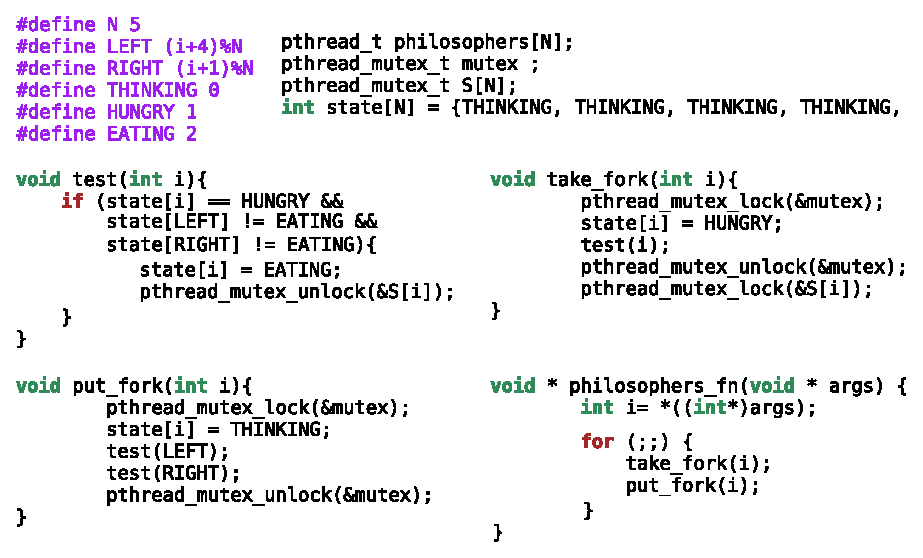
\includegraphics[width=0.55\textwidth]{media/philosophers.pdf}
    \caption{Philosophers example program}
    \label{fig:philosophers}
\end{figure*}

\begin{figure}[t!]
\centering
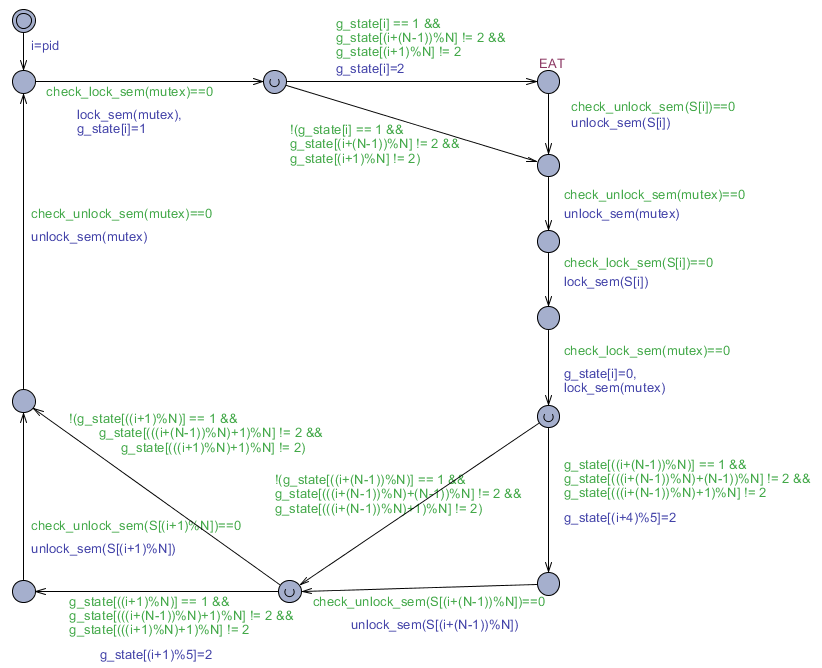
\includegraphics[width=\columnwidth]{media/uppaal_filos.png}
\caption{Philosophers diagram}
\label{fig:uppaal_philo}
\end{figure}


The program is executed in the symbolic execution framework which provides a set of paths that covers all possible transitions in the timed automaton. Once the program is symbolically executed and the automatons have been obtained (see Figure \ref{fig:uppaal_philo}), we have queried UPPAAL the following questions, whose verification times and consumed memory can be seen in Table \ref{tab:results}:



\begin{itemize}
    \item A[] !deadlock: Verifies that for every possible path and every possible interleavings, there's never an state in which no transition is possible. It checks the absence of deadlocks. 
    \item A[] forall(i:pid) Philosopher(i).EAT imply !Philosopher((i+1)\%N).EAT \&\& !Philosopher((i+(N-1))\%N).EAT: Verifies that two neighbour philosophers do not eat simultaneously. In the dining philosophers problem, the philosophers share forks with his neighbours. Because of this, they can not eat simultaneously. This verifies the  mutual exclusion property. 
\end{itemize}

\begin{table*}[hb!]
\centering
\caption{Time and memory consumption to verify different queries in the philosophers example}
\begin{tabular}{l|c|c}
\multicolumn{3}{c}{First version}                                                                                   \\
query & time & RAM memory                                                                                       \\\hline
\verb+A[] not deadlock+                                                            &  1,747.434 s  & 44,349,240 KB  \\
\verb+A[] not (Philosopher(0).EAT and Philosopher(1).EAT)+                         &  1,064.81 s   & 44,363,828 KB  \\
\verb+A[] Philosopher(0).EAT imply !Philosopher(1).EAT && !Philosopher(4).EAT+     &  450.73 s     & 44,363,852 KB  \\
\multicolumn{3}{c}{Templated version}                                                                        \\
query & time & RAM memory                                                                                       \\\hline
\verb+A[] not deadlock+                                                           &  0.65 s        & 18,564 KB     \\
\verb+A[] not (Philosopher(0).EAT and Philosopher(1).EAT)+                        &  0.227 s       & 18,628 KB     \\
\verb+A[] Philosopher(0).EAT imply !Philosopher(1).EAT && !Philosopher(4).EAT+    &  0.48 s        & 18,628 KB     \\
\end{tabular}
\label{tab:results}
\end{table*}


\section{Results}

In order to evaluate the proposed methodology, we have translated the program shown in Figure \ref{fig:philosophers} with the described tool. Two experiments have been performed whose results are shown in Table \ref{tab:results}. In the `first\_version' section, the raw output of the tool is evaluated. In this experiment, the tool has generated five templates with twelve states each, corresponding to the several instantiations of diagram shown in Figure \ref{fig:uppaal_philo}. In the second experiment, the automata have been manually parametrized generating a single template with five instantiations, in which we vary the `identifier' parameter. As we can see in Table \ref{tab:results}, the verification times and used memory are heavily reduced considering this transformation. In section `future work', this optimization is proposed as a way to reduce the verification complexity. Both experiments have been evaluated with UPPAAL 4.1.19 over a host computer with 8 Intel Xeon E5-2687W at 3.10 GHz. Every processor has 8 cores, thus the host platform integrates 64 cores running Fedora-Linux with kernel 3.16.2-201. The computer also has 64 GB of RAM. All the checked properties are satified. 



\section{Conclusions and future work}

The tool presented in this article is capable of translating generic C programs to UPPAAL timed automatons if the user provides information about which functions can be potentially running in parallel in the system. Some ongoing and future work is focused on obtaining this information automatically, which implies a previous symbolic execution step in which all pointers passed to the `pthread\_create' functions are analysed so the possible values that they can take (and therefore the possible functions that can be called) can be automatically deduced.

Another ongoing activity focuses on modeling the synchronzation element. As noticed in \cite{cicirelli2011}, different ways of modeling the synchronization primitives in UPPAAL produce drastic improvements in verification time. We have focused in both legibility and generality as the two main targets, but being able to detect the use of richer schemes and abstract the internals of the synchronizations can be useful to verify larger concurrent systems. As usually the synchronization primitives are reused and programmers rely on their correctness, the verification time can be reduced if the behaviour of these parts of the system can be abstracted.

We can also see in Table \ref{tab:results} that verification time and memory increase drastically when the same template is replicated statically instead  of providing a parameter to model different instantiations. Although this transformation has been perfomed manually in this case, it is easy to be automated, and is being done actually in the tool.

\begin{thebibliography}{1}

\bibitem{philo_1}
W. Stallings, Operating Systems: Internals and Design Principles.
Upper Saddle River, NJ, USA: Prentice Hall Press, 2005.

\bibitem{philo_2}
A. Silberschatz, P. Galvin, and G. Gagne, Operating System Concepts,
8th ed. Wiley Publishing, 2008.

\bibitem{philo_3}
A. S. Tanenbaum, Modern Operating Systems. Upper Saddle River,
NJ, USA: Prentice Hall Press, 2001.

\bibitem{tctl_1}
Thomas A. Henzinger. Symbolic model checking for real-time systems. Information
and Computation, 111:193–244, 1994.

\bibitem{tctl_2}
Rajeev Alur, Costas Courcoubetis, and David L. Dill. Model-checking for real-
time systems. In 5th Symposium on Logic in Computer Science (LICS'90), pages 414–425, 1990.

\bibitem{cicirelli2011}
Cicirelli, F., Nigro, L., \& Pupo, F. (2011). Modelling And Verification Of Concurrent Programs Using UPPAAL. ECMS, 2011, 525-533.

\bibitem{forest_tacas}
P.Gonzalez-de-Aledo, P.Sanchez. ``Framework for embedded system verification'', in Proc. of the 21th International Conference on Tools and Algorithms for the Construction and Analysis of Systems (TACAS), 2015.

\bibitem{pedersen}
PEDERSEN, J. K. A. M. S. Automatic Translation from UPPAAL to C.

\bibitem{hendriks01}
M. Hendriks, “Translating UPPAAL to Not Quite C,” Computing Science Institute, Tech. Rep. CSI-R0108, 2001.


\bibitem{amnell04}
Amnell, T., Fersman, E., Mokrushin, L., Pettersson, P., \& Yi, W. (2004). TIMES: a tool for schedulability analysis and code generation of real-time systems. In Formal Modeling and Analysis of Timed Systems (pp. 60-72). Springer Berlin Heidelberg.

\bibitem{pajik11}

Pajic, M., Lee, I., Mangharam, R., \& Sokolsky, O. (2011). UPP2SF: Translating UPPAAL models to Simulink. University of Pennsylvania, Tech. Rep.


\bibitem{cicirelli13}
Cicirelli, F., Furfaro, A., Nigro, L., \& Pupo, F. (2013, September). Modelling Java concurrency: An approach and a UPPAAL library. In Computer Science and Information Systems (FedCSIS), 2013 Federated Conference on (pp. 1373-1380). IEEE.

\bibitem{uppaal}
Automatic Verification of Real-Time Communicating Systems by Constraint Solving. Wang Yi, Paul Pettersson and Mats Daniels. In Proceedings of the 7th International Conference on Formal 
Description Techniques, Berne, Switzerland, 4-7 October, 1994.

\bibitem{cbmc}
Clarke, E., Kroening, D., \& Lerda, F. (2004). A tool for checking ANSI-C programs. In Tools and Algorithms for the Construction and Analysis of Systems (pp. 168-176). Springer Berlin Heidelberg.

\bibitem{sage} Godefroid, P., Levin, M. Y., \& Molnar, D. (2012). SAGE: whitebox fuzzing for security testing. Queue, 10(1), 20.

\bibitem{llvm}
Lattner, C., \& Adve, V. (2004, March). LLVM: A compilation framework for lifelong program analysis \& transformation. In Code Generation and Optimization, 2004. CGO 2004. International Symposium on (pp. 75-86). IEEE.

\end{thebibliography}


\end{document}


